\chapter{Конструкторская часть}

В данном разделе представлены этапы проектирования системы: функциональная модель, диаграмма базы данных и архитектуры приложения.

\section{Функциональная модель}

На рисунке \ref{img:func_model} изображена функциональная модель, отображающая структуру и функции системы.

\begin{figure}[h!]
	\begin{center}
		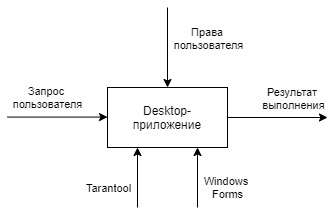
\includegraphics[scale=0.6]{../imgs/func_model.jpg}
	\end{center}
	\captionsetup{justification=centering}
	\caption{Функциональная модель приложения}
	\label{img:func_model}
\end{figure}









\section{Проектирование базы данных}


В соответствии с ER-диаграммой системы, изображенной на рисунке \ref{img:er}, база данных должна хранить следующие таблицы:  


\begin{itemize}
	\item таблица трасс slopes;
	\item таблица подъемников lifts;
	\item таблица связей трасс и подъемников lifts\_slopes;
	\item таблица турникетов turnstiles;
	\item таблица проездных карт cards;
	\item таблица считываний карт на турникетах подъемников card\_readings;
	\item таблица сообщений о происшествиях messages;
	\item таблица пользователей users.
	%\item таблица групп пользователей.
\end{itemize}


На рисунке \ref{img:db} представлена диаграмма разрабатываемой базы данных.

\begin{figure}[h!]
	\begin{center}
		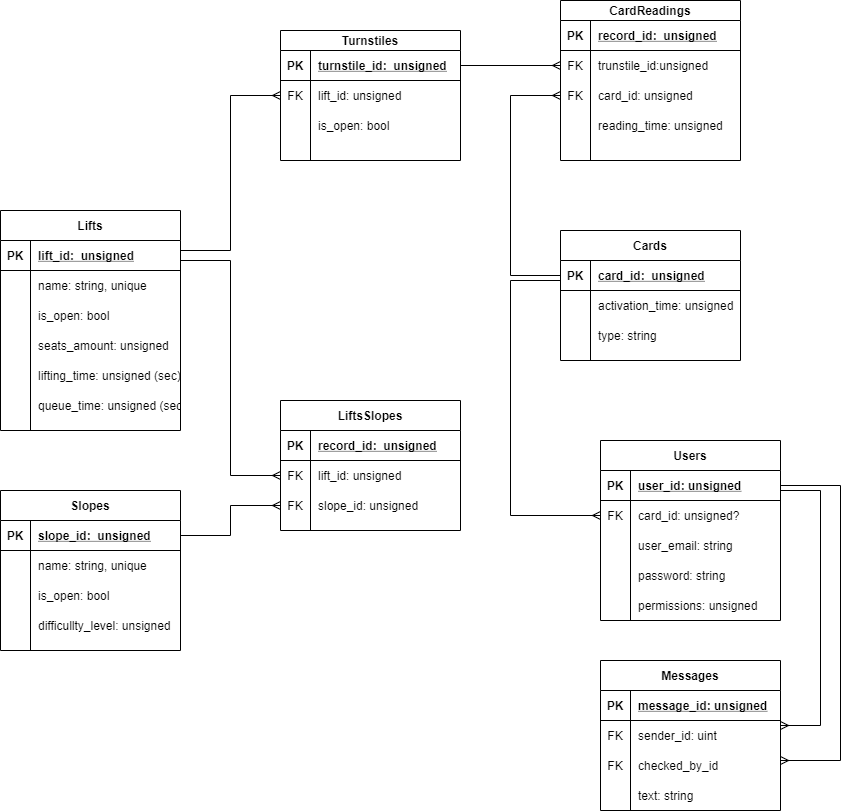
\includegraphics[scale=0.4]{../imgs/db/db.png}
	\end{center}
	\captionsetup{justification=centering}
	\caption{Диаграмма базы данных}
	\label{img:db}
\end{figure}

Таблица slopes хранит информацию о трассах и содержит следующие поля:
\begin{itemize}
	\item slope\_id -- уникальный идентификатор трассы, PK (первичный ключ, англ. primary key), unsigned;
	\item slope\_name -- уникальное название, string;
	\item difficulty\_level -- уровень сложности, unsigned;
	\item is\_open -- открыта или закрыта, boolean.
\end{itemize}


Таблица lifts хранит информацию о подъемниках и содержит следующие поля:
\begin{itemize}
	\item lift\_id -- уникальный идентификатор подъемника, PK, unsigned;
	\item lift\_name -- уникальное название, string;
	\item is\_open -- открыт или закрыт, boolean;
	\item seats\_amount -- количество мест, unsigned;
	\item lifting\_time -- время подъема в секундах, unsigned;
	\item queue\_time -- время в очереди в секундах, unsigned;
\end{itemize}


Таблицы slopes и lifts связаны отношением многие-ко-многим. Таблица lifts\_slopes хранит информацию об этом отношении (связи трасс и подъемников) и содержит следующие поля:
\begin{itemize}
	\item record\_id -- уникальный идентификатор записи, PK, unsigned;
	\item lift\_id -- идентификатор подъемника, FK на поле lift\_id таблицы lifts, unsigned;
	\item slope\_id -- идентификатор трассы, FK на поле slope\_id таблицы slopes, unsigned.
\end{itemize}


Таблица turnstiles хранит информацию о турникетах и содержит следующие поля:
\begin{itemize}
	\item turnstile\_id -- уникальный идентификатор турникета, PK, unsigned;
	\item lift\_id -- идентификатор подъемника, на котором установлен этот турникет, FK на поле lift\_id таблицы lifts, unsigned;
	\item is\_open -- открыт или закрыт, boolean.
\end{itemize}


Таблица cards хранит информацию о проездных картах и содержит следующие поля:
\begin{itemize}
	\item card\_id -- уникальный идентификатор карты, PK, unsigned;
	\item activation\_time -- дата и время активации в формате Unix-time (количество секунд, прошедших с полуночи (00:00:00 UTC) 1 января 1970 года), unsigned;
	\item type -- тип карты, string.
\end{itemize}


Таблица card\_readings хранит информацию о считываниях карт на турникетах подъемников и содержит следующие поля:
\begin{itemize}
	\item record\_id -- уникальный идентификатор считывания, PK, unsigned;
	\item turnstile\_id -- идентификатор турникета, на котором произошло считывание, FK на поле turnstile\_id таблицы turnstiles, unsigned;
	\item card\_id -- идентификатор проездной карты, которая прошла считывание, FK на поле card\_id таблицы cards, unsigned;
	\item reading\_time -- дата и время считывания в формате Unix-time, unsigned.
\end{itemize}


Таблица users хранит информацию о пользователях и содержит следующие поля:
\begin{itemize}
	\item user\_id -- уникальный идентификатор пользователя, PK, unsigned;
	\item card\_id -- идентификатор проездной карты, которая принадлежит пользователю (может отсутствовать), FK на поле card\_id таблицы cards, unsigned;
	\item user\_email -- адрес электронной почты (он же будет использоваться как логин), string;
	\item password -- пароль, string;
	\item permissions -- права доступа (роль), unsigned.
\end{itemize}


Таблица messages хранит информацию о сообщениях пользователей о происшествиях и содержит следующие поля:
\begin{itemize}
	\item message\_id -- уникальный идентификатор сообщения, PK, unsigned;
	\item sender\_id -- идентификатор отправителя, FK на поле user\_id таблицы usres, unsigned;
	\item checked\_by\_id -- идентификатор прочитавшего, FK на поле user\_id таблицы usres, unsigned;
	\item text -- текст сообщения, string.	
\end{itemize}


\section{Проектирование архитектуры приложения}

Интерфейс для работы с базой данных представляет собой  многокомпонентное desktop-приложение. На базовом уровне выделены три компонента: компонент доступа к данным, компонент бизнес-логики и компонент реализации пользовательского интерфейса. На рисунке \ref{img:components} представлена архитектура приложения.

\begin{figure}[h!]
	\begin{center}
		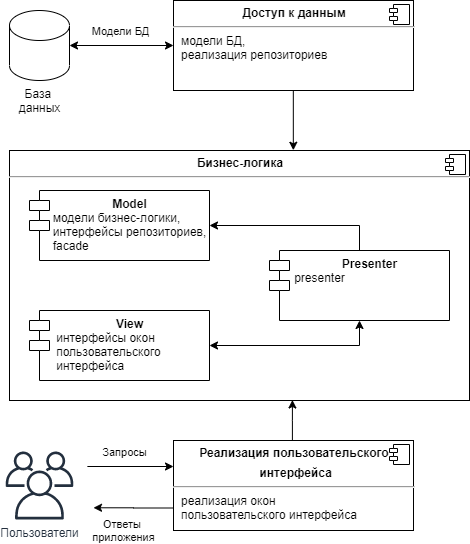
\includegraphics[scale=0.7]{../imgs/uml/components.png}
	\end{center}
	\captionsetup{justification=centering}
	\caption{Архитектура приложения}
	\label{img:components}
\end{figure}

Компонент бизнес-логики спроектирован по схеме MVP (Model-View-Presenter) и является главным (независимым). Он отвечает за логику обработки запросов и данных.

Компонент доступа к данным отвечает за получение данных из БД, их изменение, добавление и удаление. Для его реализации использован паттерн <<репозиторий>>. 

Компонент реализации пользовательского интерфейса предоставляет реализацию UI для выбранного технологического стека.

\section{Алгоритм расчета времени в очереди на подъемник}\label{func_label}



%1) как лучше назвать этот подпункт 

%2) должен ли он быть здесь (так как обычно схемы в конструкторской части), или стоит перенести схему в 3.3.2, прям перед реализацией этой функции (и как лучше назвать сам этот пункт 3.3.2, а то <<реализация функций>> тоже звучит не очень)


Для онлайн-мониторинга очередей на подъемниках необходимо реализовать функцию update\_queue\_time, которая будет обновлять время в очереди к каждому из них. Эта функция будет периодически, через некоторый заданный интервал времени, вызываться из приложения для каждого подъемника из БД. 

На рисунке \ref{img:function} представлены схемы алгоритмов функции \\update\_queue\_time и вспомогательной функции count\_card\_readings, которая возвращает количество считываний на указанном подъемнике в заданный промежуток времени.

\clearpage
\begin{figure}[h!]
	\begin{center}
		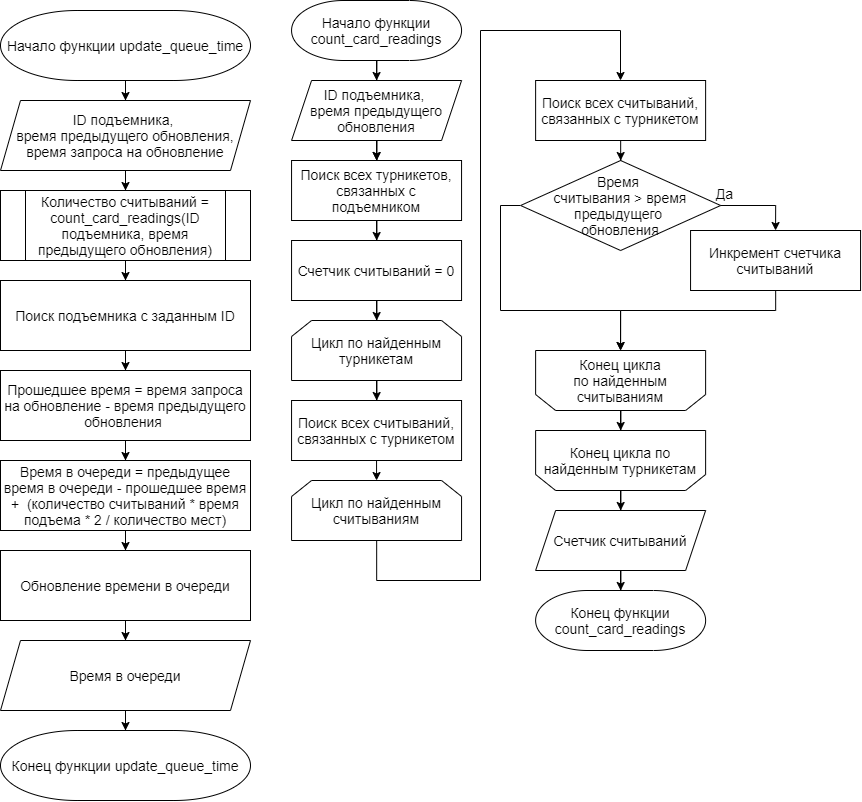
\includegraphics[scale=0.5]{../imgs/function.png}
	\end{center}
	\captionsetup{justification=centering}
	\caption{Схема работы алгоритма функции update\_queue\_time}
	\label{img:function}
\end{figure}


\section*{Вывод}

В данном разделе была приведена функциональная модель системы, спроектирована база данных и архитектура приложения, приведена схема работы алгоритма расчета времени в очереди на подъемниках.




